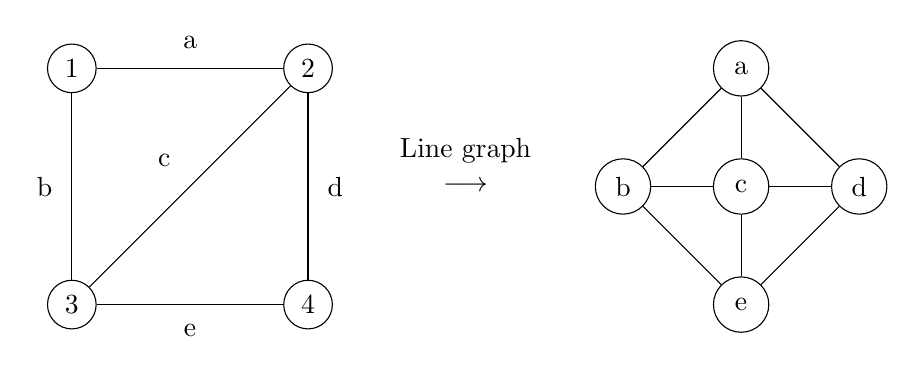
\begin{tikzpicture}[black/.style={circle,draw,fill=black,inner sep=0pt, minimum width=4pt}]
\node[circle,draw] at (0,3) (1) {1};
\node[circle,draw] at (3,3) (2) {2};
\node[circle,draw] at (0,0) (3) {3};
\node[circle,draw] at (3,0) (4) {4};

\draw (1) -- (2) node [midway,label=above:{a}] {};
\draw (1) -- (3) node [midway,label=left:{b}] {};
\draw (2) -- (3) node [midway,label=above left:{c}] {};
\draw (2) -- (4) node [midway,label=right:{d}] {};
\draw (3) -- (4) node [midway,label=below:{e}] {};


\draw node at (5, 1.5) {$\longrightarrow$};
\draw[above,yshift=5] node at (5,1.5) {Line graph};


\node[circle,draw,minimum width=20pt] at (8.5,3) (a) {a};
\node[circle,draw,minimum width=20pt] at (7,1.5) (b) {b};
\node[circle,draw,minimum width=20pt] at (8.5,1.5) (c) {c};
\node[circle,draw,minimum width=20pt] at (10,1.5) (d) {d};
\node[circle,draw,minimum width=20pt] at (8.5,0) (e) {e};

\draw (a) -- (b);
\draw (a) -- (c);
\draw (a) -- (d);
\draw (b) -- (c);
\draw (b) -- (e);
\draw (c) -- (d);
\draw (c) -- (e);
\draw (d) -- (e);
\end{tikzpicture}
